\section{Хранение посылок и результатов тестирования}

Необходимо было разработать способ уменьшить нагрузку на ФС.
На файловой системе хранился код посылок пользователей,
протоколы и результаты тестирования.
Можно выделить следующие кейсы, нагружающие ФС (все кейсы значительно нагружают ФС из-за наличия десятков миллионов маленьких файлов, делая доступ к файлу медленным):

\begin{enumerate}
    \item Оправка посылки -- Master-ejudge сохраняет отправленные посылки в ФС для дальнейшего их тестирования Инвокерами.
    \item Сохранения протоколов и результатов тестирования -- Инвокеры после тестирования посылки отправляют сохраняют их на ФС.
    \item Просмотр посылки -- при просмотре исходного кода пользователем py-ручки берут его из ФС.
    \item Просмотр протокола и результатов тестирования -- при просмотре протокола и результатов тестирования py-ручки берут их из ФС.
    \item Бэкапы данных о посылках и протоколах.
\end{enumerate}

Так вносить изменения в работу ejudge -- дорого и нетривиально, 
нагрузка, даваемая пунктами а и б может быть уменьшена единственным способом:
уменьшением количества сохранённых таким образом на ФС файлов.

Для того, чтобы удалить файлы из ФС, 
не потеряв при этом исходники посылок пользователей и их протоколы, 
необходимо предварительно сохранить файлы из ФС в другое хранилище.
Это хранилище может быть реализовано с помощью одной из существующих СУБД.
В таком случае, маленькие файлы могут храниться внутри больших блобов (англ. Binary Large Object — двоичный большой объект).

Проблемы в и г также решаются введением нового хранилища:
результаты тестирования и посылки, запрашиваемые пользователями будут доставаться из нового хранилища.

Скорость доступа к ним может быть в таком случае увеличена с использованием индексов.

В качестве ключа индекса будет использован идентификатор посылки новой таблицы pynfornatics.runs, id (подробнее описано в главе \ref{lab:pynformatics_run_id}).

Проблему с бэкапами можно решить следующим способом:
во-первых, нагрузка на ФС и так уменьшится из-за бэкапа блобов, а не маленьких файлов, 
во-вторых, если выбранная СУБД будет иметь возможность создания реплик, 
можно будет создать одну из таких реплик на другом сервере, синхронизируя её с основным экземпляром через сеть Интернет, и делать бекапы на нём. 
В таком случае, нагрузка на ФС основного сервера при проведении бекапов расти не будет.

Необходимо отметить, что протоколы тестирования по своей структуре -- 
плохо структурированные небольшие файлы, которые можно представить в виде набора JSON-ов.
В качестве хранилища для исходников и протоколов была выбрана СУБД MongoDB, так как она хорошо подохдит дляхранения плохо структурированных данных\cite{mongo_good_for_unstruct}.

MongoDB (от англ. humongous — огромный) -- документоориентированная СУБД с открытым исходным кодом, не требующая описания схемы таблиц. 
MongoDB классифицирована как NoSQL, и использует JSON-подобные документы и схему базы данных. 
MongoDB (с дефолтным движком WiredTiger\cite{mongo_store_engine}) хранит данные в блобах\cite{mongo_wiredtiger}, поддерживает индексирование и имеет функционал репликации\cite{mongo_indexes}\cite{mongo_replicas}.

Для хранения данных в MongoDB были использованы следующие схемы:

\begin{itemize}
    \item protocol -- для хранения протоколов и результатов тестирования;
    \item source -- для хранения исходного кода пользователей.
\end{itemize}

Сохранить существующие данные с ФС в MongoDB -- тривиально,
но что делать с новыми протестированными посылками?
В новой архитектуре Информатикс уже есть сервис, 
который знает, что посылка протестировалась -- это ejudge-listener (подробнее описан в главе \ref{lab:ejudge_listener}).

Для сохранения новых протестированных посылок, 
функциональность сервиса ejudge-listener была расширена 
-- при получении обновлении посылки ejudge-listener теперь забирает протокол посылки и результат тестирования из ФС и сохраняет в MongoDB.

\begin{figure}
  \centering
  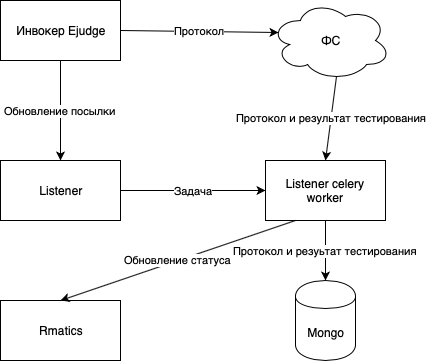
\includegraphics[width=\textwidth]{figures/listener.png}
  \caption{Схема работы ejudje-listener}
  \label{fig:ejudge_listener}
\end{figure}

